%% Definitioner för LIPS-dokument

\usepackage[swedish]{babel}
\usepackage[utf8]{inputenc}
\usepackage[T1]{fontenc}
\usepackage{times}
\usepackage{ifthen}

\usepackage[margin=25mm]{geometry}

\def\arraystretch{1.6}

\usepackage{fancyhdr}
\pagestyle{fancy}
\lhead{}
\chead{\LIPSprojekttitel}
\rhead{\LIPSdatum}
\lfoot{\LIPSkursnamn \\ \LIPSdokumentansvarig}
\rfoot{\LIPSprojektgrupp \\ \LIPSgruppepost}

\setlength{\parindent}{0pt}
\setlength{\parskip}{1ex plus 0.5ex minus 0.2ex}


\newcommand{\twodigit}[1]{\ifthenelse{#1<10}{0}{}{#1}}
\newcommand{\dagensdatum}{\number\year-\twodigit{\number\month}-\twodigit{\number\day}}

%% ------------------------------------------
% NYBILD
% Skapar centrerad bild med caption
%   
% #1: Filens url relativt '/bilder/'
% #2:  Caption
% #3: Label
% #4: Skalning i förhållande till textwidth
%% ------------------------------------------
\newcommand{\nyBild}[4] 
{\begin{figure}[H]
  \centering
 \includegraphics[angle=0,width=#4\textwidth]{bilder/#1}
  \emph{\caption{#2} \label{fig:#3}}
  
\end{figure}}

%%  Redefinitions of commands containing @
\makeatletter
\makeatother

\newcommand{\LIPStitelsida}{%
{\ }\vspace{45mm}
\begin{center}
  \textbf{\Huge {\sffamily \LIPSdokumenttyp}}
  
  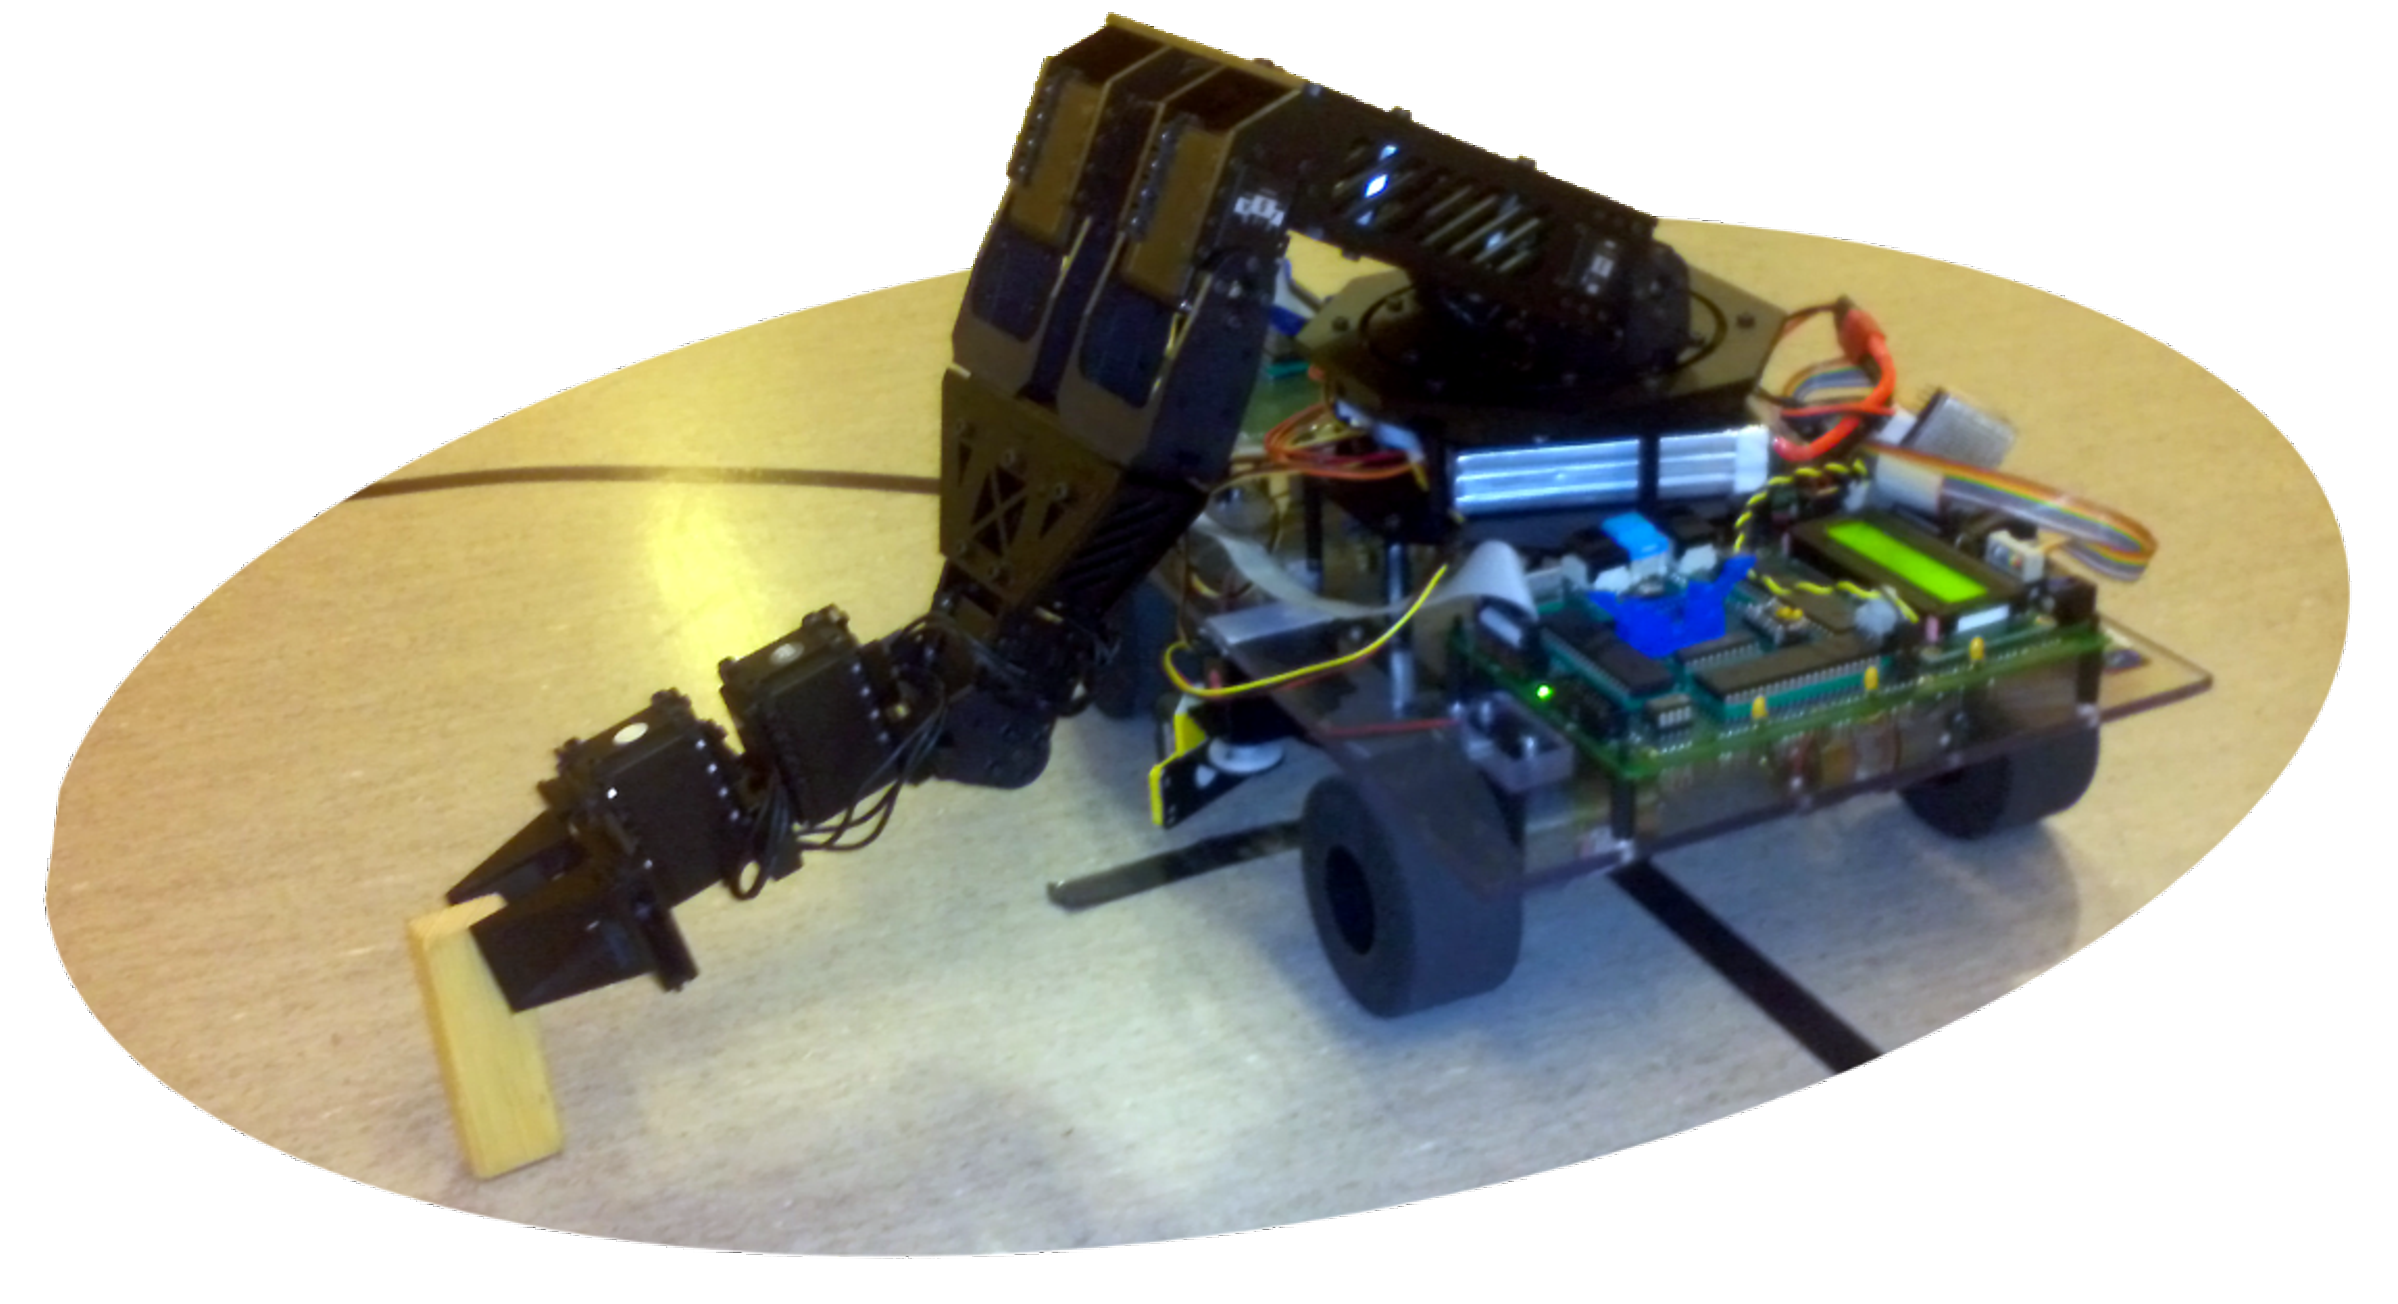
\includegraphics[width=0.8\textwidth]{../Kappa/bilder/introbild.pdf}
\end{center}
\begin{center}
  {\Large Redaktör: \LIPSredaktor}
\end{center}
\begin{center}
  {\Large Version \LIPSversion}
\end{center}
\vspace{20mm}
\begin{center}
  {\large Status}\\[1.5ex]
  \begin{tabular}{|*{3}{p{40mm}|}}
    \hline
    Granskad & \LIPSgranskare & \LIPSgranskatdatum \\
    \hline
    Godkänd & \LIPSgodkannare & \LIPSgodkantdatum \\
    \hline
  \end{tabular}
\end{center}
\newpage
}


\newenvironment{LIPSprojektidentitet}{%
{\ }\vspace{45mm}
\begin{center}
  {\Large PROJEKTIDENTITET}\\[0.5ex]
  {\small
  \LIPSprojektgrupp, \LIPSartaltermin, \LIPSprojekttitel\\
  Linköpings tekniska högskola, ISY
  }
\end{center}
\begin{center}
  \begin{tabular}{|l|p{45mm}|p{25mm}|l|}
    \hline
    \textbf{Namn} & \textbf{Ansvar} & \textbf{Telefon} & \textbf{E-post} \\
    \hline
}
{
    \hline
  \end{tabular}
\end{center}
\begin{center}
  {\small
    \textbf{E-postlista för hela gruppen}: \LIPSgruppepost\\
    \textbf{Kontaktperson hos kund}: \LIPSkundkontakt\\
    \textbf{Kursansvarig}: \LIPSkursansvarig\\
    \textbf{Handledare}: \LIPShandledare\\
  }
\end{center}
\newpage
}
\newcommand{\LIPSgruppmedlem}[4]{\hline {#1} & {#2} & {#3} & {#4} \\}



\newenvironment{LIPSdokumenthistorik}{%
\begin{center}
  Dokumenthistorik\\[1ex]
  \begin{small}
    \begin{tabular}{|l|l|p{60mm}|l|l|}
      \hline
      \textbf{Version} & \textbf{Datum} & \textbf{Utförda förändringar} & \textbf{Utförda av} & \textbf{Granskad} \\
      }%
    {%
      \hline
    \end{tabular}
  \end{small}
\end{center}
}
\newcommand{\LIPSversionsinfo}[5]{\hline {#1} & {#2} & {#3} & {#4} & {#5} \\}



\newenvironment{packed_itemize}{
\begin{itemize}
	\setlength{\itemsep}{1pt}
    \setlength{\parskip}{0pt}
    \setlength{\parsep}{0pt}
}{\end{itemize}}

\newenvironment{packed_enumerate}{
\begin{enumerate}
	\setlength{\itemsep}{1pt}
    \setlength{\parskip}{0pt}
    \setlength{\parsep}{0pt}
}{\end{enumerate}}





%%% Local Variables: 
%%% mode: latex
%%% TeX-master: "kravspec_mall"
%%% End: